\documentclass[../../../../main.tex]{subfiles}
\begin{document}

\begin{flushright}
\footnotesize\textit{【自動文字起こし・要確認】}
\end{flushright}

[解] $p = t+1$ とおいて全て書きかえる
$$ \begin{cases} x = \frac{(p-1)^2(4-p)}{p} = x(p) \\ y = \frac{(p-1)^3(4-p)}{p} = y(p) \end{cases} \quad (1 \le p \le 4) $$
より
$$ \begin{cases} x'(p) = x(p) \frac{4-p^2}{(p-1)(4-p)p} = \frac{4-p^2}{p^2} \\ y'(p) = y(p) \frac{-2(p^2-2p-2)}{(p-1)(4-p)p} = \frac{-2(p-1)(p^2-2p-2)}{p^2} \end{cases} $$
区間内で $x, y \ge 0$ より、下表をうる
\begin{center}
\begin{tabular}{|c|c|c|c|c|c|c|c|}
\hline
$p$ & $1$ & $\cdots$ & $2$ & $\cdots$ & $1+\sqrt{3}$ & $\cdots$ & $4$ \\
\hline
$x'$ & & $+$ & $0$ & $-$ & & $-$ & \\
\hline
$y'$ & & $+$ & & $+$ & $0$ & $-$ & \\
\hline
$(x, y)$ & $(0, 0)$ & $\nearrow$ & $(1, 1)$ & $\nwarrow$ & $(\frac{3}{2}(1-\sqrt{3})^2, \frac{\sqrt{3}}{2}(1-\sqrt{3})^3)$ & $\swarrow$ & $(0, 0)$ \\
\hline
\end{tabular}
\end{center}
これと $x(p) \le y(p) \iff 2 \le p$ ($\because 1 \le p \le 4$) から、グラフは右下図。
したがって、
$$ \begin{cases} 0 \le x \le 1 \\ 0 \le y \le 3(-3+2\sqrt{3}) \end{cases} $$
又、右図斜線部の面積 $S$ は
\begin{align*}
S &= \int_0^1 y dx - \frac{1}{2} \\
S + \frac{1}{2} &= \int_4^1 \frac{(p-1)^3(4-p)}{p} \cdot \frac{4-p^2}{p^2} dp \\
&= \int_4^1 \frac{p^5 - 6p^4 + 5p^3 + 20p^2 - 36p + 16}{p^3} dp \\
&= \int_4^1 \left( p^2 - 6p + 5 + \frac{20}{p} - \frac{36}{p^2} + \frac{16}{p^3} \right) dp \\
&= \left[ \frac{1}{3}p^3 - 3p^2 + 5p + 20 \log p + \frac{36}{p} - \frac{8}{p^2} \right]_4^1 \\
&= -\frac{63}{3} + 3 \cdot 15 - 15 - 40 \log 2 + 27 - \frac{15}{2} \\
&= 36 - 40 \log 2 - \frac{15}{2}
\end{align*}
$$ S = 28 - 40 \log 2 $$

\begin{center}
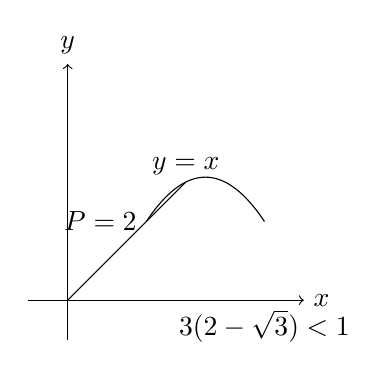
\begin{tikzpicture}
\draw[->] (-0.5,0) -- (3,0) node[right]{$x$};
\draw[->] (0,-0.5) -- (0,3) node[above]{$y$};
\draw[domain=0:1.5, smooth] plot (\x, {\x});
\node at (1.5, 1.7) {$y=x$};
\draw[domain=1:2.5, smooth] plot ({\x}, {-\x*\x+3.5*\x-1.5}); 
\node at (1, 1) [left] {$P=2$};
\node at (2.5, 0) [below] {$3(2-\sqrt{3})<1$};
\end{tikzpicture}
\end{center}

\end{document}
